\section{Mismatch between beta-distribution and cumulative density distribution for peaks.\label{mismatch}}

The prevalence of activation of the peaks are overestimated in the simulations.  This is mainly due to the mismatch between the beta distribution with which we modeled the alternative peaks, and the observed cumulative density distribution for peaks.  To illustrate we have plotted in Figure \ref{fig.mismatch} the estimated beta-distribution that is fitted to the alternative peaks, and the observed cumulative distribution based on the estimated effect sizes.
For the former, we have calculated the average location parameter of the beta-distribution from \citet{Pounds2004} for the different conditions.  We have plotted these beta-distributions in the left plot of Figure \ref{fig.mismatch}.
For the latter, we have simulated $10^8$ values following the estimated truncated normal distribution.  For each of these values, we have calculated the $p$-value following Equation 2 in the main manuscript.  The resulting density of these values are plotted in the right plot of Figure \ref{fig.mismatch}.
It can be seen that the distributions are more similar for small effect sizes, but as the effect size increases, so does the mismatch.  This explains why smaller sample sizes have less bias than larger sample sizes.

\begin{center}
\begin{figure}
  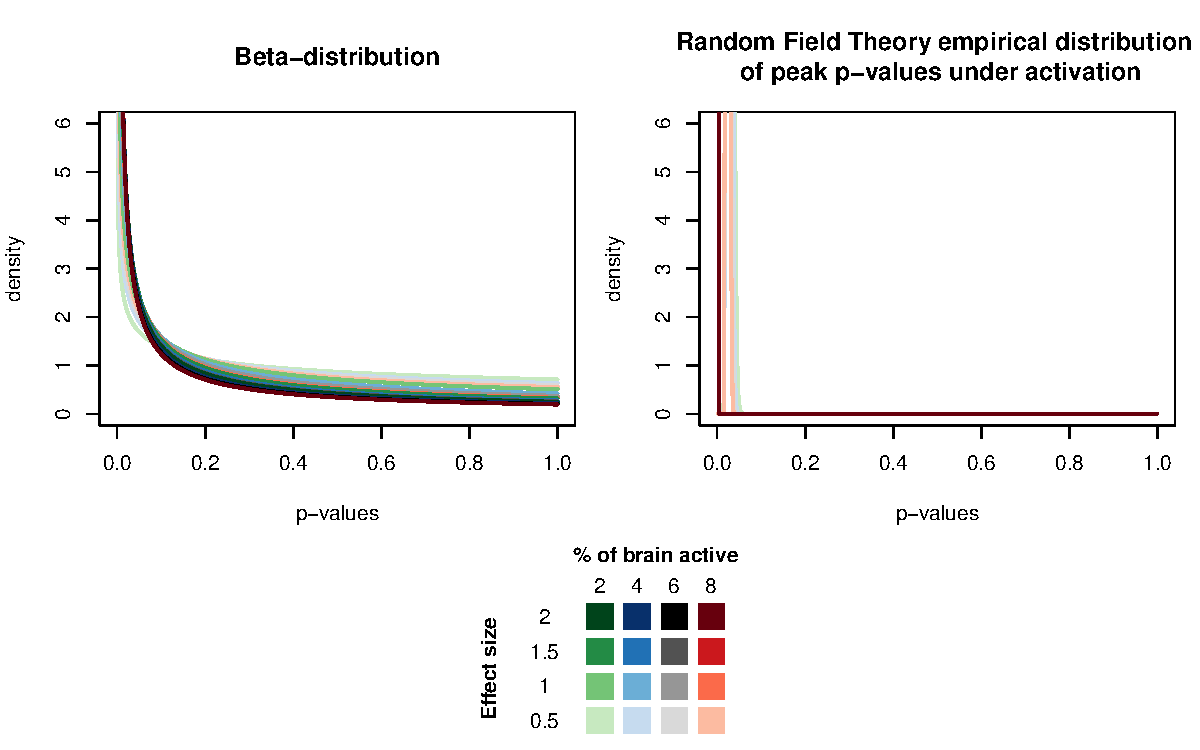
\includegraphics[scale=0.8]{FIG_SIM_distribution_mismatch.pdf}
  \caption{Plot of estimated beta-distributions and expected distributions \label{fig.mismatch}}
\end{figure}
\end{center}
